\documentclass[12pt]{article}
\usepackage[danish]{babel}
\usepackage{amsfonts, amssymb, mathtools, amsthm, amsmath}
\usepackage{graphicx, pgfplots}
\usepackage{url}
\usepackage[dvipsnames]{xcolor}
\usepackage{sagetex}
\usepackage{lastpage}
\usepackage{wrapfig} 
\usepackage[stretch=10]{microtype}


%loaded last
\usepackage[hidelinks]{hyperref}

\usepackage{siunitx}
  \sisetup{exponent-product = \cdot,
    output-decimal-marker = {,}}

%Giles Castelles incfig
\usepackage{import}
\usepackage{xifthen}
\usepackage{pdfpages}
\usepackage{transparent}

\newcommand{\incfig}[2][1]{%
  \def\svgwidth{#1\columnwidth}
  \import{../figures/}{#2.pdf_tex}
}

\setlength{\parindent}{0in}
\setlength{\oddsidemargin}{0in}
\setlength{\textwidth}{6.5in}
\setlength{\textheight}{8.8in}
\setlength{\topmargin}{0in}
\setlength{\headheight}{18pt}

\usepackage{fancyhdr}
\pagestyle{fancy}

\fancyhead{}
\fancyfoot{}
\fancyfoot[R]{Side \thepage{} af \pageref{LastPage}}
\fancyhead[L]{\footnotesize{Noah Rahbek Bigum Hansen}}

% Redefine the plain page style to be consistent
\fancypagestyle{plain}{
  \fancyhead{} % Clears all header content
  \fancyfoot{} % Clears all footer content
  \renewcommand{\headrulewidth}{0pt} % Removes the horizontal line
  \fancyfoot[R]{Side \thepage{} af \pageref{LastPage}} % Page number in the footer
}

\pgfplotsset{compat=newest}

\pgfplotsset{every axis/.append style={
  axis x line=middle,    % put the x axis in the middle
  axis y line=middle,    % put the y axis in the middle
  axis line style={<->,color=black}, % arrows on the axis
}}

\usepackage{thmtools}
\usepackage{tcolorbox}
  \tcbuselibrary{skins, breakable}
  \tcbset{
    space to upper=1em,
    space to lower=1em,
  }

\theoremstyle{definition}

\newtcolorbox[auto counter]{definition}[1][]{%
  breakable,
  colframe=ForestGreen,  %frame color
  colback=ForestGreen!5, %background color
  colbacktitle=ForestGreen!25, %background color for title
  coltitle=ForestGreen!70!black,  %title color
  fonttitle=\bfseries\sffamily, %title font
  left=1em,              %space on left side in box,
  enhanced,              %more options
  frame hidden,          %hide frame
  borderline west={2pt}{0pt}{ForestGreen},  %display left line
  title=Definition \thetcbcounter: #1,
}

\newtcolorbox{greenline}{%
  breakable,
  colframe=ForestGreen,  %frame color
  colback=white,          %remove background color
  left=1em,              %space on left side in box
  enhanced,              %more options
  frame hidden,          %hide frame
  borderline west={2pt}{0pt}{ForestGreen},  %display left line
}

\newtcolorbox[auto counter, number within=section]{eks}[1][]{%
  brekable,
  colframe=NavyBlue,  %frame color
  colback=NavyBlue!5, %background color
  colbacktitle=NavyBlue!25,    %background color for title
  coltitle=NavyBlue!70!black,  %title color
  fonttitle=\bfseries\sffamily, %title font
  left=1em,            %space on left side in box,
  enhanced,            %more options
  frame hidden,        %hide frame
  borderline west={2pt}{0pt}{NavyBlue},  %display left line
  title=Eksempel \thetcbcounter: #1
}

\newtcolorbox{blueline}{%
  breakable,
  colframe=NavyBlue,     %frame color
  colback=white,         %remove background
  left=1em,              %space on left side in box,
  enhanced,              %more options
  frame hidden,          %hide frame
  borderline west={2pt}{0pt}{NavyBlue},  %display left line
}

\newtcolorbox{teo}[1][]{%
  breakable,
  colframe=RawSienna,  %frame color
  colback=RawSienna!5, %background color
  colbacktitle=RawSienna!25,    %background color for title
  coltitle=RawSienna!70!black,  %title color
  fonttitle=\bfseries\sffamily, %title font
  left=1em,              %space on left side in box,
  enhanced,              %more options
  frame hidden,          %hide frame
  borderline west={2pt}{0pt}{RawSienna},  %display left line
  title=Teori: #1,
}

\newtcolorbox[auto counter, number within=section]{sæt}[1][]{%
  breakable,
  colframe=RawSienna,  %frame color
  colback=RawSienna!5, %background color
  colbacktitle=RawSienna!25,    %background color for title
  coltitle=RawSienna!70!black,  %title color
  fonttitle=\bfseries\sffamily, %title font
  left=1em,              %space on left side in box,
  enhanced,              %more options
  frame hidden,          %hide frame
  borderline west={2pt}{0pt}{RawSienna},  %display left line
  title=Sætning \thetcbcounter: #1,
  before lower={\textbf{Bevis:}\par\vspace{0.5em}},
  colbacklower=RawSienna!25,
}

\newtcolorbox{redline}{%
  breakable,
  colframe=RawSienna,  %frame color
  colback=white,       %Remove background color
  left=1em,            %space on left side in box,
  enhanced,            %more options
  frame hidden,        %hide frame
  borderline west={2pt}{0pt}{RawSienna},  %display left line
}

\newtcolorbox{for}[1][]{%
  breakable,
  colframe=NavyBlue,  %frame color
  colback=NavyBlue!5, %background color
  colbacktitle=NavyBlue!25,    %background color for title
  coltitle=NavyBlue!70!black,  %title color
  fonttitle=\bfseries\sffamily, %title font
  left=1em,              %space on left side in box,
  enhanced,              %more options
  frame hidden,          %hide frame
  borderline west={2pt}{0pt}{NavyBlue},  %display left line
  title=Forklaring #1,
}

\newtcolorbox{bem}{%
  breakable,
  colframe=NavyBlue,  %frame color
  colback=NavyBlue!5, %background color
  colbacktitle=NavyBlue!25,    %background color for title
  coltitle=NavyBlue!70!black,  %title color
  fonttitle=\bfseries\sffamily, %title font
  left=1em,              %space on left side in box,
  enhanced,              %more options
  frame hidden,          %hide frame
  borderline west={2pt}{0pt}{NavyBlue},  %display left line
  title=Bemærkning:,
}

\makeatother
\def\@lecture{}%
\newcommand{\lecture}[3]{
  \ifthenelse{\isempty{#3}}{%
    \def\@lecture{Lecture #1}%
  }{%
    \def\@lecture{Lecture #1: #3}%
  }%
  \subsection*{\makebox[\textwidth][l]{\@lecture \hfill \normalfont\small\textsf{#2}}}
}

\makeatletter

\newcommand{\opgave}[1]{%
 \def\@opgave{#1}%
 \subsection*{Opgave #1}
}

\makeatother

%Format lim the same way in intext and in display
\let\svlim\lim\def\lim{\svlim\limits}

% horizontal rule
\newcommand\hr{
\noindent\rule[0.5ex]{\linewidth}{0.5pt}
}


\title{Eksamen i Fysik og Mekanik}
\author{Noah Rahbek Bigum Hansen}
\date{16. December 2024}

\begin{document}

\maketitle

\section*{1.}
\begin{figure} [ht]
  \centering
  \caption{}
  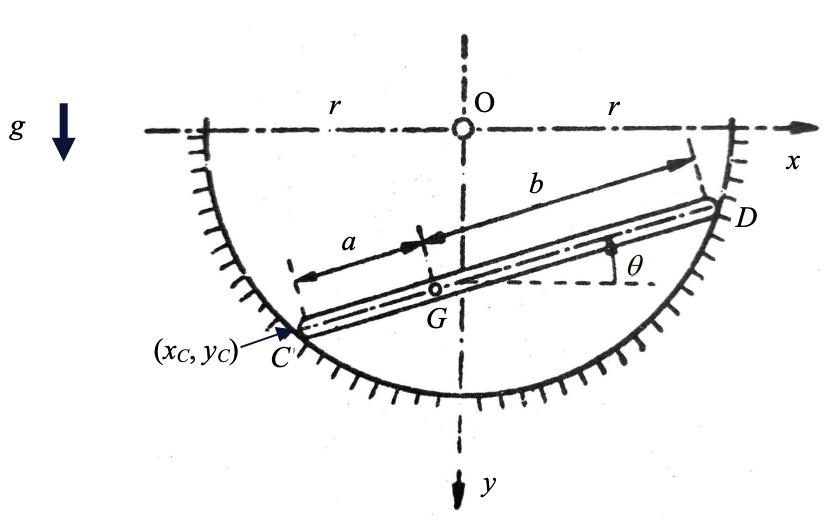
\includegraphics[width=0.35\linewidth]{../figures/E1.png}
  \label{fig:E1}
\end{figure}

En stang $CD$ med tyngdepunkt i $G$ ligger gnidningsfrit i en sfærisk skål, med radius $r$, som vist (i tværsnit) i \textbf{\autoref{fig:E1}}. Stangens længde $l = a + b$. Symbolet $g$ angiver tyngdeaccelerationen.

\subsection*{(a)}
Angiv omhyggeligt, i et frit-legeme diagram for stangen $CD$, reaktionskræfterne (el. normalkræfterne) i endepunkterne $C$ og $D$, inklusive deres retgninger.
\bigbreak
\begin{figure}[ht]
  \centering
  \incfig[0.6]{Ek1}
  \caption{Frit-legeme diagram}
  \label{fig:Ek1}
\end{figure}
På \underline{\underline{\textbf{\autoref{fig:Ek1}}}} (på næste side) ses et fritlegemediagram for stangen. Normalkræfterne vil, virke langs en normal (deraf navnet) til cirklens periferi. Derfor vil normalkræfterne begge have retning mod origo, da en normal til en cirkel altid peger mod dens centrum. Da de to kræfter begge har vinkler der ikke er lig $\theta$ kan vi ikke opstille et udtryk for deres størrelse vha. ligevægtsbetingelserne idet vinklen for hver kraft er ubekendt og derfor fås 3 ligninger med 4 ubekendte (størrelsen af $R_C$, vinklen til $R_C$, størrelsen af $R_D$ og vinklen til $R_D$).

\subsection*{(b)}
Vis så, ved at gøre brug af din besvarelse af spg. (a), at ved statisk ligevægt vil koordinaterne for endepunkt $C$ være givet ved
\[ 
  (x_c, y_c) = \left( -a \cos\theta, \sqrt{r^2 - a^2 \cos^2 \theta} \right)
,\]
hvor $\theta$ er vinklen mellem stangen $CD$ og vandret (se \textbf{\autoref{fig:E1}}). (Bemærk at ordinaten $y$ er positiv nedad!)
Vink: Vi har, for punktet $(x_c, y_c)$ beliggende på halvcirklen (\textbf{\autoref{fig:E1}}), at $x_c^2 + y_c^2 = r^2$.
\bigbreak
Idet det antages, at der ikke er friktion må det gælde, at massemidtpunktet i situationen med statisk ligevægt vil have placeret sig så lavt som muligt (dette er den laveste energitilstand). Dermed fås at afstanden $a$ kommer til at være afstanden fra $C$ til $y$-aksen langs stangen. Vi kan derfor med trigonometri finde $x$-koordinatet som
\[
  \cos \theta = \frac{x_C}{-a} \implies x_c = -a \cos\theta
.\]
Vi har fra pythagoras læresætning at
\[ 
x_C^2 + y_C^2 = r^2 \implies y_c = \sqrt{r^2 - x_C^2} = \sqrt{r^2 - a^2 \cos^2 \theta}
.\]
Altså er det vist at \underline{\underline{$(x_c, y_c) = (-a \cos\theta, \sqrt{r^2 - a^2 \cos^2 \theta})$}}.


\section*{2.}
\begin{figure} [ht]
  \centering
  \caption{}
  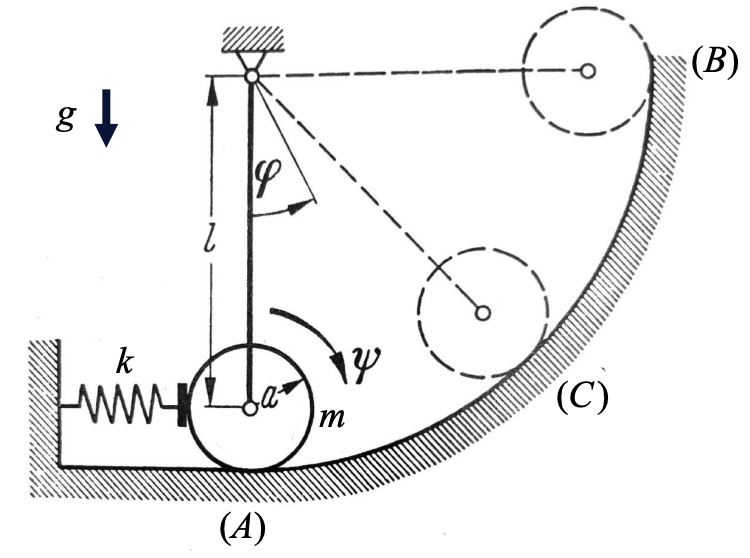
\includegraphics[width=0.5\linewidth]{../figures/E2.png}
  \label{fig:E2}
\end{figure}

En masseløs stang med længde $l$ er ophængt i et friktionsfrit leje i den ene ende og er forsynet med en massiv cylinder, med radius $a$ og masse $m$, i den anden ende. Lejet, som forbinder cylinder og stav, kan ligeledes antages at være friktionsfrit. Stangens position beskrives ved vinklen $\phi$, medens cylinderens ”drejningsvinkel” beskrives ved vinklen $\psi$. (se \textbf{\autoref{fig:E2}}). Når stangen er i lodret position (A), påvirkes cylinderen af en masseløs fjeder med fjederkonstanten $k$. Med andre ord, fjederen er monteret sådan, at den er sammentrykt, og påvirker cylinderen med en kraft, når vinklen $\phi = 0$ (se \textbf{\autoref{fig:E2}}). Det antages, at cylinderen, efter frigivelse, ruller op ad den kvartcirkelformede banekurve uden at glide. Tyngdeaccelerationen er $g$. 

\subsection*{(a)}
Bestem sammenhængen mellem vinklerne $\phi$ og $\psi$.
\bigbreak
Vi kan finde den instantane vinkelhastighed for stangen som
\[ 
\omega = \lim_{\Delta t \to 0} \frac{\Delta \phi}{\Delta t} = \frac{\mathrm{d}\phi}{\mathrm{d}t} 
.\]
Vinkelhastighed er relateret til den tangentielle hastighed som
\[ 
v_{tan} = l\omega
.\]
Vi har dermed at den tangentielle hastighed for stangen er
\[ 
v_{tan} = l \frac{\mathrm{d}\phi}{\mathrm{d}t} 
.\]
Stangens tangentielle hastighed må tilsvare hastigheden af cylinderens massemidtpunkt $v_{cm}$. Altså har vi
\[ 
v_{cm} = v_{tan} = l \frac{\mathrm{d}\phi}{\mathrm{d}t} 
.\]
Idet det antages at der ikke er en glidning mellem banekurven og cylinderen er hastigheden af cylinderens massemidtpunkt $v_{cm}$ relateret til dens vinkelhastighed $\frac{\mathrm{d}\psi}{\mathrm{d}t}$ som
\[ 
v_{cm} = a \cdot \frac{\mathrm{d}\psi}{\mathrm{d}t} 
.\]
Vi får altså
\begin{align*}
  a \frac{\mathrm{d}\psi}{\mathrm{d}t} &= l \frac{\mathrm{d}\phi}{\mathrm{d}t}  \\
  a \psi &= l \phi
.\end{align*}
Dermed har vi at sammenhængen mellem de to vinkler er \underline{\underline{$a\psi = l\phi$}}


\subsection*{(b)}
Hvor stort et stykke $x$ skal fjederen være sammentrykt ved stangposition (A) ($\phi = 0$) for at stangen (med cylinder), når den frigives bevæger sig op til -- og stopper ved -- den vandrette stangposition (B)?
\bigbreak
Idet der er energibevarelse må det gælde at
\[ 
k_{A} + U_{A} = k_{B} + U_{B}
.\]
Idet cylinderen hverken har en hastighed ved $A$ eller ved $B$ reduceres det ovenstående til
\[ 
U_{A} = U_B
.\]
Al den potentielle energi i begyndelsespositionen $A$ kommer fra den potentielle energi lagret i fjederen og alt den potentielle energi i slutpositionen $B$ er gravitational potentiel energi. Vi får altså at
\begin{align*}
  U_{A} &= \frac{1}{2}kx^2 \\
  U_{B} &= mgh
.\end{align*}
Højden $h$ til slutpositionen er i øvrigt lig længden af stangen $l$ idet cylinderens massemidtpunkt netop flytter sig en afstand lig $l$ lodret opad mellem $A$ og $B$. Hvis de to udtryk kombineres fås altså at
\begin{align*}
  \frac{1}{2}kx^2 &= mgl \\
  x^2 &= \frac{2mgl}{k} \\
  |x| &= \sqrt{\frac{2mgl}{k}}
.\end{align*}
Altså skal fjederen sammenpresses en afstand der svarer til $|x|$, dette er i den negative retning idet koordinatsystemet placeres således, at den positive $x$-retning er mod højre. Altså skal fjederen i alt sammenpresses med en afstand \underline{\underline{$x = -\sqrt{\frac{2mgl}{k}}$}}.

\subsection*{(c)}
Hvad er stangens vinkelhastighed, $\mathrm{d}\phi / \mathrm{d}t$, når den, på vej op, passerer midt-positionen (C) (det vil sige, $\phi = \pi / 4$)?
Vink: Cylinderens masseinertimoment, $I$, er givet ved $I = \frac{1}{2}ma^2$.
\bigbreak
Vi har igen energibevarelse og dermed fås
\[ 
k_{A} + U_{A} = k_{C} + U_{C}
.\]
Igen har vi ingen hastighed i begyndelsespositionen $A$ og dermed reduceres det ovenstående til
\[ 
U_{A} = k_C + U_C
.\]
Idet stangen ikke har nogen masse er al den kinetiske energi ved position $C$ den samlede kinetiske energi af cylinderen. Denne består både af et bidrag fra dens translatoriske kinetiske energi og af et bidrag fra den rotationelle potentielle energi. Denne er altså
\[ 
k_C = \frac{1}{2}mv_{cm}^2 + \frac{1}{2}I_{cm}\omega_{\phi}^2 = \frac{1}{2}m v_{cm}^2 + \frac{1}{2} \left( \frac{1}{2}ma^2 \right)\omega^2
.\]
Dette kan simplificeres til
\begin{align*}
  k_C &= \frac{1}{2}m v_{cm}^2 + \frac{1}{4}ma^2\omega^2 \\
  &= \frac{1}{2}m v_{cm}^2 + \frac{1}{4}m v_{cm}^2\\
  &= \frac{3}{4} m v_{cm^2}
.\end{align*}
Højden af cylinderens massemidtpunkt til $\phi = \pi / 4$ kan findes vha. trigonometri som
\[ 
h = l \cos\phi
.\]
Dermed bliver den gravitationelle potentielle energi ved punkt $C$
\[ 
U_C = mg l \cos\phi
.\]
Den potentielle energi ved $A$ er tidligere fundet til at være
\[ 
U_A = \frac{1}{2}kx^2
.\]
Vi kan dermed kombinere udtrykkene som
\begin{align*}
  \frac{1}{2}kx^2 = \frac{3}{4}m v_{cm}^2 + mgl \cos\phi
.\end{align*}
Heri kan $v_{cm}$ isoleres som
\begin{align*}
  \frac{3}{4} m v_{cm}^2 &= \frac{1}{2}kx^2 - mgl \cos \phi \\
  m v_{cm}^2 &= \frac{2}{3} kx^2 - \frac{4}{3} mgl \cos \phi \\
  v_{cm} &= \sqrt{\frac{\frac{2}{3}kx^2}{m} - \frac{4}{3}gl \cos\phi} \\
.\end{align*}
Vi har tidligere vist at stangens vinkelhastighed $\mathrm{d}\phi / \mathrm{d}t \cdot l = v_{cm}$. Det ovenstående kan altså omskrives til
\[ 
\frac{\mathrm{d}\phi}{\mathrm{d}t} l = \sqrt{\frac{\frac{2}{3}kx^2}{m} - \frac{4}{3}gl \cos\phi} \implies \frac{\mathrm{d}\phi}{\mathrm{d}t} = \frac{\sqrt{\frac{\frac{2}{3}kx^2}{m} - \frac{4}{3}gl \cos\phi}}{l}
.\]
Det ovenstående kan simplificeres som
\begin{align*}
  \frac{\mathrm{d}\phi}{\mathrm{d}t} &= \frac{\sqrt{\frac{\frac{2}{3}kx^2}{m} - \frac{4}{3}gl \cdot \frac{1}{2} \sqrt{2}}}{l} \\      
  &= \frac{\sqrt{\frac{2}{3}\left( \frac{kx^2}{m} - \sqrt{2}gl \right)}}{l}
.\end{align*}
Dermed er et udtryk for stangens vinkelhastighed \underline{\underline{$\mathrm{d}\phi / \mathrm{d}t = \frac{\sqrt{\frac{2}{3}\left( \frac{kx^2}{m} - \sqrt{2}gl \right)}}{l}$}} fundet.


\section*{3.}
\begin{figure} [ht]
  \centering
  \caption{}
  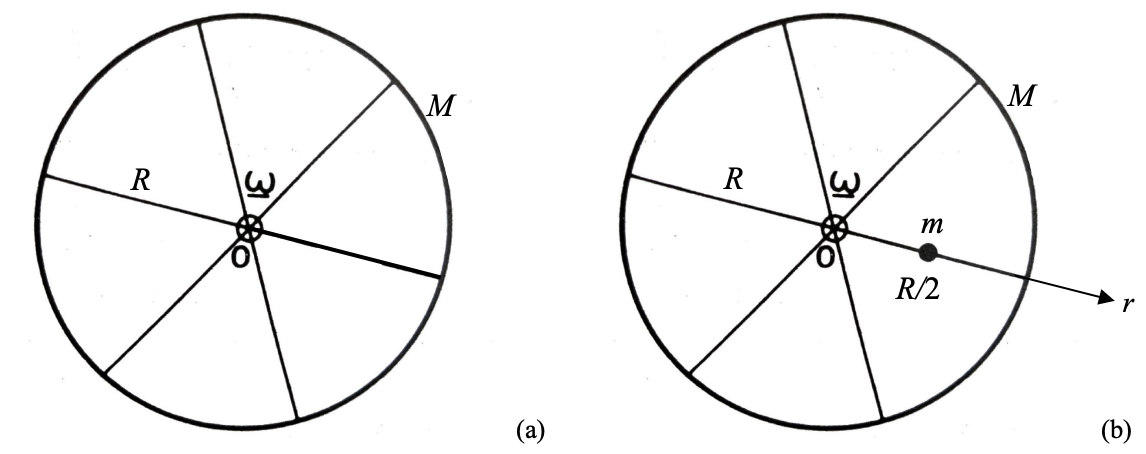
\includegraphics[width=0.5\linewidth]{../figures/E3.png}
  \label{fig:E3}
\end{figure}

En tynd, homogen ring med masse $M$ og radius $R$ roterer om en lodret akse, der er vinkelret på ringens plan og går gennem ringens centrum $O$; se \textbf{\autoref{fig:E3} (a)}. Vinkelhastigheden, $\omega$, holdes konstant i alle spørgsmål. Betragtet som en vektor peger $\omega$ op, ud af papirets plan. Egerne, som forbinder ringen med et leje i dens centrum og omdrejningspunkt $O$, kan antages at være masseløse. Der kan ses bort fra tyngdekraften. 

\subsection*{(a)}
Find den kraft, der virker i et snit i ringen.
Vink: Optegn (omhyggeligt) et frit-legeme diagram for en halv ring, og påfør snitkræfterne (normalkræfterne) $F$ i snittene. Bestem da $F$ ved dynamisk ligevægt.
\bigbreak
\begin{figure}[ht]
  \centering
  \incfig[0.3]{Ek2}
  \caption{Fritlegemediagram}
  \label{fig:Ek2}
\end{figure}
I toppen af ringen vil snittet blive påvirket (``skubbet'') af den anden halvdel af ringen og i bunden af ringen vil snittet blive påvirket af en modsatrettet kraft (``trukket'') af den anden halvdel af ringen. Eftersom der er dynamisk ligevægt må det gælde at summen af kræfter og kraftmomenter er 0. Altså har vi at
\begin{align*}
  \sum F &= 0 \\
  \sum \tau &= 0
.\end{align*}
Det ovenstående kan omskrives til
\[ 
F - F = 0 
\]
og
\[ 
F R - FR = 0
.\]
Af begge disse udtryk kan ses at den samlede kraft, der virker i et snit i ringen altså er \underline{\underline{$\sum F = 0$}}.

\subsection*{(b)}
Ringen forsynes nu med en lille masse $m$, anbragt i afstanden $R / 2$ fra centrum, se \textbf{\autoref{fig:E3} (b)}. Bestem systemets impulsmoment (eng.: angular momentum) om rotationsaksen, samt dets kinetiske energi.
\bigbreak
Idet egerne er masseløse må ringens inertimoment være tilsvarende inertimomentet for en hul cylinder, altså
\[ 
I_{r} = MR^2
.\]
Den lille masse regnes for en punktmasse og har derfor ikke et inertimoment om sit eget massemidtpunkt. Dens inertimoment om ringens massemidtpunkt kan fra parallel-akse-teoremet bestemmes som
\begin{align*}
  I_{m} &= I_{m_{cm}} + md^2 \\
  I_{m} &= 0 + m \frac{R^2}{4}
.\end{align*}
Det samlede inertimoment for systemet er da blot summen af disse to inertimomenter. Altså
\begin{align*}
  I_{tot} &= I_r + I_m \\
  &= MR^2 + m\frac{R^2}{4} \\
  &= R^2 \left( M + \frac{m}{4} \right)
.\end{align*}
Det samlede inertimoment \underline{\underline{$I_{tot} = R^2 \left( M + \frac{m}{4} \right)$}}.

\subsection*{(c)}
Til tiden $t = 0$ svigter den mekanisme, som fastholder massen $m$, hvorefter den glider gnidningsfrit langs egerne ud mod ringen. Vis at massens radiale position $r(t)$, til tiden $t$ (og indtil den rammer ringen), er givet ved
\[ 
r(t) = \frac{R}{4}\left( e^{\omega t} + e^{- \omega t} \right)
.\]
Vink: Opstil bevægelsesligningen (dvs., Newtons 2. lov) for massen $m$ i et koordinatsystem som roterer med ringen om $O$. Eftervis så, at det ovenfor angivne udtryk for $r(t)$ opfylder denne ligning samt begyndelsesbetingelserne $r(0) = \frac{R}{2}, v(0) = \frac{\mathrm{d}r(0)}{\mathrm{d}t} = 0$.
\bigbreak
De afledede af den givne ligning er
\begin{align*}
  \frac{\mathrm{d}r}{\mathrm{d}t} &=\frac{R}{4} \, {\left(\omega e^{\omega t} - \omega e^{-\omega t}\right)}\\
  \frac{\mathrm{d}^2 r}{\mathrm{d}t^2} &= \frac{R}{4} \, {\left(\omega^{2} e^{\omega t} + \omega^{2} e^{-\omega t}\right)}
.\end{align*}


Vi starter med at vise at det givne udtryk opfylder begyndelsesbetingelserne. For initialpositionsbetingelsen har vi
\begin{align*}
  r(0) &= \frac{R}{4}\left( e^{\omega \cdot 0} + e^{-\omega \cdot 0}\right) \\
  &= \frac{R}{4}\cdot 2 \\
  &= \frac{R}{2}
.\end{align*}
Altså er det vist, at \underline{\underline{$r(0) = \frac{R}{2}$}}.

For initialhastighedsbetingelsen har vi at
\begin{align*}
  \frac{\mathrm{d}r(0)}{\mathrm{d}t} &= \frac{R}{4} \left( \omega e^{\omega \cdot 0} - \omega e^{-\omega 0} \right) \\
  &= \frac{R}{4}\cdot (1-1) \\
  &= 0
.\end{align*}
Altså er det ligeledes vist, at \underline{\underline{v(0) = 0}}.

For at undersøge om den givne ligning opfylder bevægelsesligningen skal bevægelseslignignen først opskrives. Vi har generelt Newtons 2. lov for et roterende referencesystem som
\[ 
m \ddot{r} = \Vec{F} + 2m \dot{r} \times \Vec{\Omega} + m \left( \Vec{\Omega}\times \Vec{r} \right)\times \Vec{\Omega}
.\]
Sættes $\Omega = \omega$ og vi husker at der ikke er nogen kraft der påvirker massen $m$ i inertialsystemet bliver det ovenstående til
\[ 
m \frac{\mathrm{d}^2 r}{\mathrm{d}t^2} = 2m \frac{\mathrm{d}r}{\mathrm{d}t} \times\omega + m \left( \Vec{\omega} \times \Vec{r} \right) \times \Vec{\omega} \implies \frac{\mathrm{d}^2 r}{\mathrm{d}t^2} = 2 \frac{\mathrm{d}r}{\mathrm{d}t}\times\omega + \left( \Vec{\omega} \times \Vec{r} \right) \times \Vec{\omega}
.\]
Idet der til ethvert tidspunkt er \ang{90} grader mellem $\Vec{\omega}$ og $\Vec{r}$ reduceres det ovenstående til
\[ 
\frac{\mathrm{d}^2r}{\mathrm{d}t^2} = 2 \frac{\mathrm{d}r}{\mathrm{d}t}\omega + \omega^2 \cdot r
.\]
Vi ønsker nu at vise at det givne udtryk for $r(t)$ opfylder den fundne bevægelsesligning. Vi får at
\begin{align*}
  \frac{R}{4} \left( \omega^2 e^{\omega t} + \omega^2 e^{-\omega t} \right) &= \frac{R}{2}\left( \omega e^{\omega t} - \omega e^{-\omega t} \right)\omega + \omega^2 \cdot \frac{R}{4}(e^{\omega t} + e^{-\omega t}) \\
  \frac{R\omega^2}{4}\left( e^{\omega t} + e^{-\omega t} \right) &= \frac{R\omega^2}{2} \left( e^{\omega t} - e^{-\omega t} \right) + \frac{R\omega^2}{4} \left( e^{\omega t} + e^{-\omega t} \right)\\
  \frac{1}{4} \left( e^{\omega t} + e^{-\omega t} \right) &= \frac{1}{2} \left( e^{\omega t} - e^{-\omega t} \right) + \frac{1}{4} \left( e^{\omega t} + e^{-\omega t} \right) \\
  \frac{1}{4}e^{\omega t} + \frac{1}{4}e^{-\omega t} &= \frac{1}{2} e^{\omega t} - \frac{1}{2} e^{-\omega t} + \frac{1}{4} e^{\omega t} + \frac{1}{4} e^{-\omega t} \\
  \frac{1}{2}e^{\omega t} + \frac{1}{2}e^{-\omega t} &= e^{\omega t} - e^{-\omega t} + \frac{1}{2}e^{\omega t} + \frac{1}{2}e^{-\omega t}  \\
  \frac{1}{2}e^{\omega t} + \frac{1}{2}e^{-\omega t} &= \frac{3}{2} e^{\omega t} - \frac{1}{2}e^{-\omega t}
.\end{align*}
Der er sket en fortegnsfejl et sted i det ovenstående idet resultat ikke er det forventede.


\subsection*{(d)}
Idet massens bevægelse beskrives i et roterende koordinatsystem, som angivet i spg. (c), ønskes angivet størrelse og retning af de fiktive kræfter som påvirker partiklen, når den befinder sig i afstanden $r$ fra $O$ ($R / 2 < r < R$). 
\bigbreak
De to fiktive kræfter der virker på partiklen er hhv. centrifugalkraften og corioliskraften. Disse er generelt givet som
\begin{align*}
  \Vec{F}_{cor} &= 2m \dot{r} \times \omega \\
  \Vec{F}_{cf} &= m \left( \Vec{\omega} \times \Vec{r} \right) \times \Vec{\omega}
.\end{align*}
Idet der altid er \ang{90} mellem vinkelhastighedsvektoren $\Vec{\omega}$ og stedvektoren $\Vec{r}$ reduceres de to ovenstående ligninger til
\begin{align*}
  F_{cor} &= 2m \frac{R}{4} \left( \omega e^{\omega t} - \omega e ^{-\omega t} \right) \\
  F_{cp} &= m \cdot \omega^2 \cdot \frac{R}{4} \left( e^{\omega t} + e^{-\omega t} \right)
.\end{align*}
Bemærk at i det ovenstående er $F_{cor} = |\Vec{F}_{cor}|$ og $F_{cp} = |\Vec{F}_{cp}|$. Altså er udtryk for størrelsen af de fiktive kræfter fundet til \underline{\underline{$|F_{cor}| = 2m \frac{R}{4} \left( \omega e^{\omega t} - \omega e^{-\omega t}\right)$}} og \underline{\underline{$|F_{cp}| = m \omega^2 \frac{R}{4} \left( e^{\omega t} + e^{-\omega t} \right)$}}. Vi har fra højrehåndsreglen, at retningen af \underline{\underline{$F_{cor}$ altid er vinkelret mod højre for partiklen}} idet den bevæger sig væk fra rotationens midtpunkt og vha. højrehåndsreglen kan det ligeledes ses at retningen af centrifugalkraften \underline{\underline{$F_{cf}$ altid vil være vinkelret væk fra omdrejningspunktet}}.


\end{document}
